\documentclass[12pt]{article}
\usepackage[top=1in, bottom=1in, left=.75in, right=.75in]{geometry}
\usepackage{amsmath,cmbright,coordsys}
\usepackage{fancyhdr}
\usepackage{graphicx}
\usepackage{txfonts}
\usepackage{multicol}
\usepackage{wrapfig}
\usepackage[scaled=0.86]{helvet}
\usepackage{anyfontsize}
% \usepackage{times}
% \usepackage[lf]{MinionPro}
\usepackage{tikz,pgfplots}

\usepackage{textcomp,enumerate}

\renewcommand{\emph}[1]{\textsf{\textbf{#1}}}

\def\degC{{}^\circ{\rm C}}
\def\ra{\rightarrow}

\newcommand{\blank}[1]{\rule{#1}{0.75pt}}

% \setmainfont{Times}
% \def\sansfont{Lucida Grande Bold}
\parindent 0pt
\parskip 4pt
\pagestyle{fancy}
\fancyfoot[C]{\emph{\thepage}}
\fancyhead[L]{\ifnum \value{page} > 1\relax\emph{Math 251: Final Exam}\fi}
\fancyhead[R]{\ifnum \value{page} > 1\relax\emph{April 27, 2022}\fi}
\headheight 15pt
\renewcommand{\headrulewidth}{0pt}
\renewcommand{\footrulewidth}{0pt}
\let\ds\displaystyle
\def\continued{{\emph {Continued....}}}
\def\continuing{{\emph {Problem \arabic{probcount} continued....}}\par\vskip 4pt}


\newcounter{probcount}
\newcounter{subprobcount}
\newcommand{\thesubproblem}{\emph{\alph{subprobcount}.}}
\def\problem#1{\setcounter{subprobcount}{0}%
\addtocounter{probcount}{1}{\emph{\arabic{probcount}.\hskip 1em(#1)}}\par}
\def\subproblem#1{\par\hangindent=1em\hangafter=0{%
\addtocounter{subprobcount}{1}\thesubproblem\emph{#1}\hskip 1em}}
\def\probskip{\vskip 10pt}
\def\medprobskip{\vskip 2in}
\def\subprobskip{\vskip 45pt}
\def\bigprobskip{\vskip 4in}

\begin{document}
{\emph{\fontsize{26}{28}\selectfont Math F251\hfill
{\fontsize{32}{36}\selectfont Final Exam}
\hfill Spring 2022}}
\vskip 0.5cm
\strut\vtop{\halign{\emph#\hskip 0.5em\hfil&#\hbox to 2in{\hrulefill}\cr
\emph{\fontsize{18}{22}\selectfont Name:}&\cr}}
\hfill
\vtop{\halign{\emph{\fontsize{18}{22}\selectfont #}\hfil& \emph{\fontsize{18}{22}\selectfont\hskip 0.5ex $\square$ #}\hfil\cr
Section: & F01 (Faudree)\cr
\noalign{\vskip 4pt}
         & F02 (Gossell)\cr
\noalign{\vskip 4pt}
         & UX1 (Gossell)\cr}}

{\fontsize{18}{22}\selectfont\emph{Rules:}}

You have 2 hours to complete the exam.  

Partial credit will be awarded, but you must show your work.

No other aids are permitted.

Place a box around your  \fbox{FINAL ANSWER} to each question where appropriate.

Turn off anything that might go beep during the exam.
\vskip 0.5cm


\begin{center}
{
\sf\fontsize{16pt}{22pt}\selectfont
\renewcommand{\arraystretch}{0.8}
\begin{tabular}{|c|c|c|}
\hline
Problem & Possible & Score \\ \hline
1 & 8 & \\ \hline
2 &  8& \\ \hline
3 & 12 & \\ \hline
4 & 8& \\ \hline
5 &10 & \\ \hline
6 & 8 & \\ \hline
7 & 4 & \\ \hline
8 & 10 & \\ \hline
9 & 12 & \\ \hline
10 & 10 & \\ \hline
11 & 10 & \\ \hline
Extra Credit& 5 & \\ \hline
Total & 100 & \\ \hline
\end{tabular}
}
\end{center}

\vfill
\newpage
%derivatives (new)
\problem{8 points} Find the derivative of each of the following functions. You do not need to simplify your answer.\\
\subproblem{}  $\displaystyle g(x) = \left(\ln(x)+\frac{2x}{5}\right)^4$\\



\vfill
\subproblem{} $\displaystyle f(x) = \sqrt{x} e^{3x}$\\


\vfill


%integrals (NEW)
\problem{8 points} Evaluate the definite integrals below. \textbf{Simplify} your final answers.
	\subproblem{} $ \displaystyle \int_1^2 6x - 5 \: dx$
	\vfill
	\subproblem{} $ \displaystyle \int 7(\sin x)^3 \cos x \: dx $
	\vfill


\newpage
%l'hop (NEW)
\problem{12 points} Evaluate the following limits. You must show your work to earn full credit. If you apply L'Hopital's Rule, you should indicate this.
	\subproblem{} $\displaystyle{\lim_{x\to 2} \frac{2x^2-8}{x^2-3x+2}}$
\vfill
\subproblem{}  $\displaystyle{\lim_{x\to 4} \frac{2-\sqrt{x}}{4-x}}$
\vfill
\subproblem{}  $\displaystyle{\lim_{x\to \infty} \frac{45+x-4x^2}{x^2-16}}$
\vfill
%%Linearlization NEW
\problem{8 points} 
\begin{enumerate}[a.]
	\item Find the linear approximation (also known as the linearization) of the function $f(x)=\sqrt{x}$ when $a=4$.
	\vfill
	\item Use the linear approximation to estimate $\sqrt{4.04}$. Your answer must be in the form of a decimal.
	\vfill
\end{enumerate}

\newpage



%Optimization Problem (JILL, new)
\problem{10 points} (Optimization Problem) You need to construct a 100 $\text{ft}^2$ rectangular pen for a dog. Three sides of the pen (north, east, and south) will be made of open fencing which costs \$2 per foot. To add privacy, the west side which faces the street will be made of closed fencing which costs \$14 per foot. Follow the steps below to find the dimensions of the pen that minimize the cost.
\subproblem{} Draw a diagram and label the sides.
\vfill
\subproblem{} Write an equation for the cost of the fencing in terms of a single variable.
\vfill
\subproblem{} Use Calculus to find the dimensions of the pen that \textbf{minimize} the cost. \emph{Justify} your answer.

\vfill
\newpage
%Related Rate Problem (James)
\problem{8 points} (Related Rates Problem) The volume $V$ of a spherical snowball with radius $r$ is given by the equation $\displaystyle V=\frac{4}{3}\pi r^3$.\\
The surface area $A$ is given by $\displaystyle A=4\pi r^2$. Throughout the warm spring afternoon, the snowball melts at a constant rate of $36\pi$ cubic inches per hour.
\begin{enumerate}[a.]
\item At the moment that the radius is $6$ inches, how fast is the radius decreasing? Include units in your answer.
\vspace{1in}
\item At the moment that the radius is $6$ inches, how fast is the surface area decreasing? Include units in your answer.
\vspace{2in}
\end{enumerate}
%derivative as rate of change
\problem{4 points} The number of subscribers to an internet streaming service is given by $s(t)$, where $t$ is measured in months since the company started.\\

\subproblem{} What does the statement $s'(36)=4,580$ mean? Include units with your answer.
\vfill
\subproblem{} Would the owners of the streaming service prefer $s''(36)$ to be positive or negative? Explain your reasoning.
\vfill
\newpage
%%Initial Value, velocity and acceleration (JILL)
\problem{10 points} Suppose a particle moves along a straight line with \textbf{velocity} $v(t)=3t^2-12t-2$ m/s.

\subproblem{} Find $s(t)$, the \textbf{position} of the particle at time $t$ in seconds assuming that when $t=1$ second the particle is at position $s=10$ meters.

\vfill

\subproblem{} Find $a(t),$ the \textbf{acceleration} of the particle at time $t$ in seconds.
\vfill
\subproblem{} At time $t=0,$ is the particle speeding up or slowing down? Explain your answer.
\vfill
\subproblem{} Determine the minimum velocity of the particle.
\vfill


\newpage



%derivatives + shape of graphs (James)
\problem{12 points} 
Sketch graphs which satisfy the given conditions. \textbf{There are many correct answers.}
\begin{multicols}{2}
\begin{enumerate}[a.]
\item Sketch a graph of a function $k(x)$ such that
\begin{itemize}
\item $k'(-5) > 0$
\item $k'(5) < 0$
\end{itemize}
\begin{center}
\rescaleby{1}{10}{\vlabel}
\rescaleby{1}{10}{\hlabel}
\coordsys[10][10](-75,-75)(75,75)
\end{center}

\item Sketch a graph of a function $f(x)$ that has
\begin{itemize}
\item an inflection point at $x=-5$, and
\item a local minimum at $x=5$.
\end{itemize}
\begin{center}
\rescaleby{1}{10}{\vlabel}
\rescaleby{1}{10}{\hlabel}
\coordsys[10][10](-75,-75)(75,75)
\end{center}

\item Sketch a graph of a function $g(x)$ that
\begin{itemize}
\item $\displaystyle \lim_{x \rightarrow 5^-} g(x) = 4$
\item $\displaystyle \lim_{x \rightarrow 5^+} g(x) = -2$
\end{itemize}
\begin{center}
\rescaleby{1}{10}{\vlabel}
\rescaleby{1}{10}{\hlabel}
\coordsys[10][10](-75,-75)(75,75)
\end{center}

\item Sketch a graph of a function $h(x)$ such that
\begin{itemize}
\item $h'(-5)>0$, and
\item $h''(-5)<0$.
\end{itemize}
\begin{center}
\rescaleby{1}{10}{\vlabel}
\rescaleby{1}{10}{\hlabel}
\coordsys[10][10](-75,-75)(75,75)
\end{center}



\end{enumerate}
\end{multicols}
 

\vfill

\newpage

%Given graph. questions from limits, to def of derivative, existence of derivatve, co ntinuity (JILL new)
\problem{10 points} 
\begin{multicols}{2}
Use the graph of the function $f(x)$ (on the right) to answer the questions below. 

\begin{center}
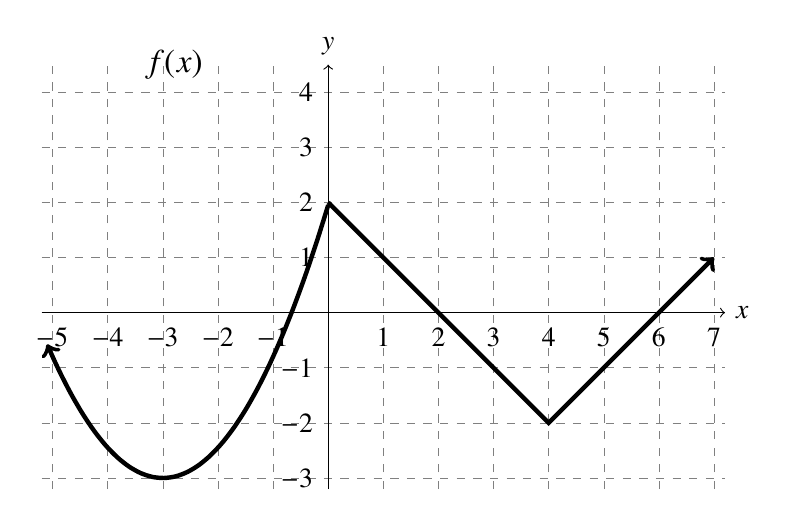
\begin{tikzpicture}[scale=.7]
\draw[help lines, dashed] (-5.2,-3.2) grid (7.2,4.5);
\draw[->] (-5.2,0) -- (7.2,0) node[right] {$x$};
\draw[->] (0,-3.2) -- (0,4.5) node[above] {$y$};
\draw  (-3.5,4.5) node[right] {\large{$f(x)$}};
\draw[ultra thick, <-] plot [smooth,domain=-5.1:0] (\x,{(.55)*(\x+3)*(\x+3)-3}); 
%\node[shape=circle, ultra thick, inner sep=1pt, draw,fill=white,minimum size=3mm] at (-2,2){};
%\node[shape=circle, ultra thick, inner sep=1pt, draw,fill=white,minimum size=3mm] at (0,3){};
%\node[shape=circle, ultra thick, inner sep=1pt, draw,fill=black,minimum size=3mm] at (-2,1){};
\draw[ultra thick, ->] (0,2) -- (4,-2)--(7,1);
%\draw[ultra thick, ->] plot [smooth] coordinates {(2,5) (3,2) (4,1) (5,1.9) (6,2.5) (7,2.75) (8,2.85) };
%\draw[style= ultra thick] (1,0) arc (0:180:1);
%\draw[style=ultra thick] (1,0) --(4,-1)--(5,0);
\foreach \x in {-5,-4,-3,-2,-1,1,2,3,4,5,6,7}
\draw (\x,-0.1) node[below] {$\x$};
\foreach \y in {-3,-2,-1,1,2,3,4}
\draw (-0.1,\y) node[left] {$\y$};
%\node[shape=circle, ultra thick, inner sep=1pt, draw,fill=white,minimum size=3mm] at (0,3){};
\end{tikzpicture}
\end{center}
\end{multicols}
\vspace*{-1in}
\subproblem{} $\displaystyle \lim_{x \to 1} f(x)=$
\vskip 0.75cm

\subproblem{} $\displaystyle \lim_{x \to 1} \frac{f(1+h)-f(1)}{h}=$
\vskip 0.75cm

\subproblem{} At what values of $x$, if any, does the derivative, $f'(x),$ not exist?
\vfill

\subproblem{} On what intervals, if any, is $f'(x)>0$?
\vfill

\subproblem{} Does $f(x)$ have any local minimums? If so, state the location and the local minimum value. \\
\vfill

The following questions concern $G(x) = \int_0^x f(s)\;ds$.
\bigskip

\subproblem{} What is the value of $G(5)$?
\vfill

\subproblem{} What is the value of $G'(5)$?
\vfill
\subproblem{} On the interval $[0,7],$ does $G(x)$ have a local minimum? If so, state the location and the local minimum value.
\vfill

\newpage


%net change (JILL NEW)
\problem{10 points}
A population of bacteria is growing at a rate of $p'(t)=300e^{t/10}$ bacteria per day. 

\subproblem{} Compute $p'(0)$ and interpret its meaning in the context of the problem. Include units with your answer.
\vspace{1in}

\subproblem{}  Compute $\displaystyle \int_0^{10} p'(t) \: dt.$
\vfill


\subproblem{} Interpret your answer from part (b) in the context of the problem. Make sure to include units.
\vfill

%\subproblem{} Does this problem contain sufficient information to be able to determine the number of bacteria on day 5? If so, explain how to find it. If not, explain what information is missing.
%\vspace{1.3in}


%%tangent line (Jill new)
%\problem{XX points}  Write an equation of the line tangent to the graph of $H(x)=x+\sin(2x)$ when $x=\pi.$
%\vfill


%%%JAMES
\problem{Extra Credit: 5 points} Calculate $\displaystyle \frac{d}{dx}\left( \int_{\cos x}^5 \frac{17^{-t}\ln(t+2)}{\sqrt{20-\sin^2 t}} \: dt \right)$.

\vfill
\end{document}
